\documentclass[12pt]{amsart}
\usepackage{geometry}
\usepackage{amsmath}
\usepackage{amssymb}
\usepackage{graphicx}
\usepackage{subfig}
\usepackage[table]{xcolor}
\usepackage{color}
\usepackage{natbib}
\usepackage{wrapfig}

\usepackage{blindtext}
\usepackage{tabularx}

\newenvironment{frcseries}{\fontfamily{frc}\selectfont}{}
\newcommand{\textfrc}[1]{{\frcseries#1}}
\newcommand{\mathfrc}[1]{\raisebox{-0.8mm}{\text{\textfrc{\small #1}}}\hspace{0.4mm}}

\geometry{letterpaper}

%\usepackage[T1]{fontenc}

% general commands
\definecolor{lemonchiffon}{rgb}{1, .98, .80}
\definecolor{lightgrass}{rgb}{.89, 1, .87}
\newcommand{\vect}[1]{\boldsymbol{\mathbf{#1}}}
\newcommand{\degree}[1]{${#1}^{\circ}$}
\newcommand{\highlight}{ \rowcolor{lightgrass} }
\newcommand{\script}[1]{\mathcal{#1}}

\newcommand{\eqn}[1]{\begin{align*}
#1
\end{align*}}
\newcommand{\eqnl}[2]{\begin{align} \label{#1}
#2
\end{align}}
\newcommand{\shblock}{\hspace{3mm}}
\newcommand{\hblock}{\hspace{8mm}}
\newcommand{\eqnsep}{\shblock\hblock}

\newcommand{\bl}{\big\{}
\newcommand{\br}{\big\}}
\newcommand{\Bl}{\Big\{}
\newcommand{\Br}{\Big\}}

\newcommand{\argmax}{\operatornamewithlimits{argmax}}

\newcommand{\indicator}{\mathbf{1}}

\newcommand{\mtx}[4]{
\[
#1 = #2
\left[ {\begin{array}{#3}
 #4
 \end{array} } \right]
\]
}

\newcommand{\eqnset}[4]{
\[ #1 = #2 \left\{ \begin{array}{#3}
        #4
\end{array} \right. \] 
}



        
        
        
        \newcommand{\img}[2]{
	\begin{figure}
		\centering
		\includegraphics[width=\textwidth]{#1}
		\caption{#2}
	\end{figure}
}

\newcommand{\imgi}[1]{
	\vspace{10mm}
	\includegraphics[width=\textwidth]{#1}
	\vspace{10mm}
}


% paper specific terms
\newcommand{\vz}{\vect{z}}
\newcommand{\vx}{\vect{x}}
\newcommand{\vy}{\vect{y}}
\newcommand{\vp}{\vect{\pi}}
\newcommand{\vph}{\hat{\vect{\pi}}}
\newcommand{\vpmle}{\hat{\vect{\pi}}_\text{MLE}}



\newcommand{\fab}{f_j}
\newcommand{\llp}{\mathfrc{l}(\vect{\pi})}

\newcommand{\pims}{1-\pi_1,\ldots,\pi_{m-1}}

\newcommand{\hessll}[2]{\sumn \frac{f_{#1}}{(\summ \pi_j f_j)^2 f_{#2}}}
\newcommand{\hessllg}[2]{\sumn \frac{f_{#1}}{(\sumg \pi_j f_j)^2 f_{#2}}}
\newcommand{\hesslld}[2]{\frac{\partial^2 \llpp}{\partial \pi_{#1} \partial \pi_{#2}}}


\newcommand{\sumn}{\sum^n_{i=1}}
\newcommand{\summ}{\sum^m_{j=1}}
\newcommand{\summo}{\sum^{m-1}_{j=1}}
\newcommand{\sumg}{\sum^g_{j=1}}
\newcommand{\sumk}{\sum^m_{k=1}}

\newcommand{\vpg}{\vp^{\prime}}
\newcommand{\vpgh}{\hat{\vp}^{\prime}}
\newcommand{\llpp}{\mathfrc{l}(\vpg)}
\newcommand{\llpph}{\mathfrc{l}(\vpgh)}


%%% TITLE
\title{Bootstrapping}
\author{\today}

%%% BEGIN DOCUMENT
\begin{document}

\maketitle

\section{Bootstrapping}
Another way to analyze the behavior of $\vph$ is to resample the data via the bootstrap. Using either parametric or non-parametric approaches, we generate $B$ bootstrap samples of $\bl (x^*_i,y^*_i) \br^n_{i=1}$, which can be run through the expectation maximization algorithm to produce $B$ bootstrapped estimates, $\vph^*_1,\ldots,\vph^*_B$.

\subsection{Parametric data generation}
\begin{wrapfigure}{r}{0.5\textwidth}
  \begin{center}
    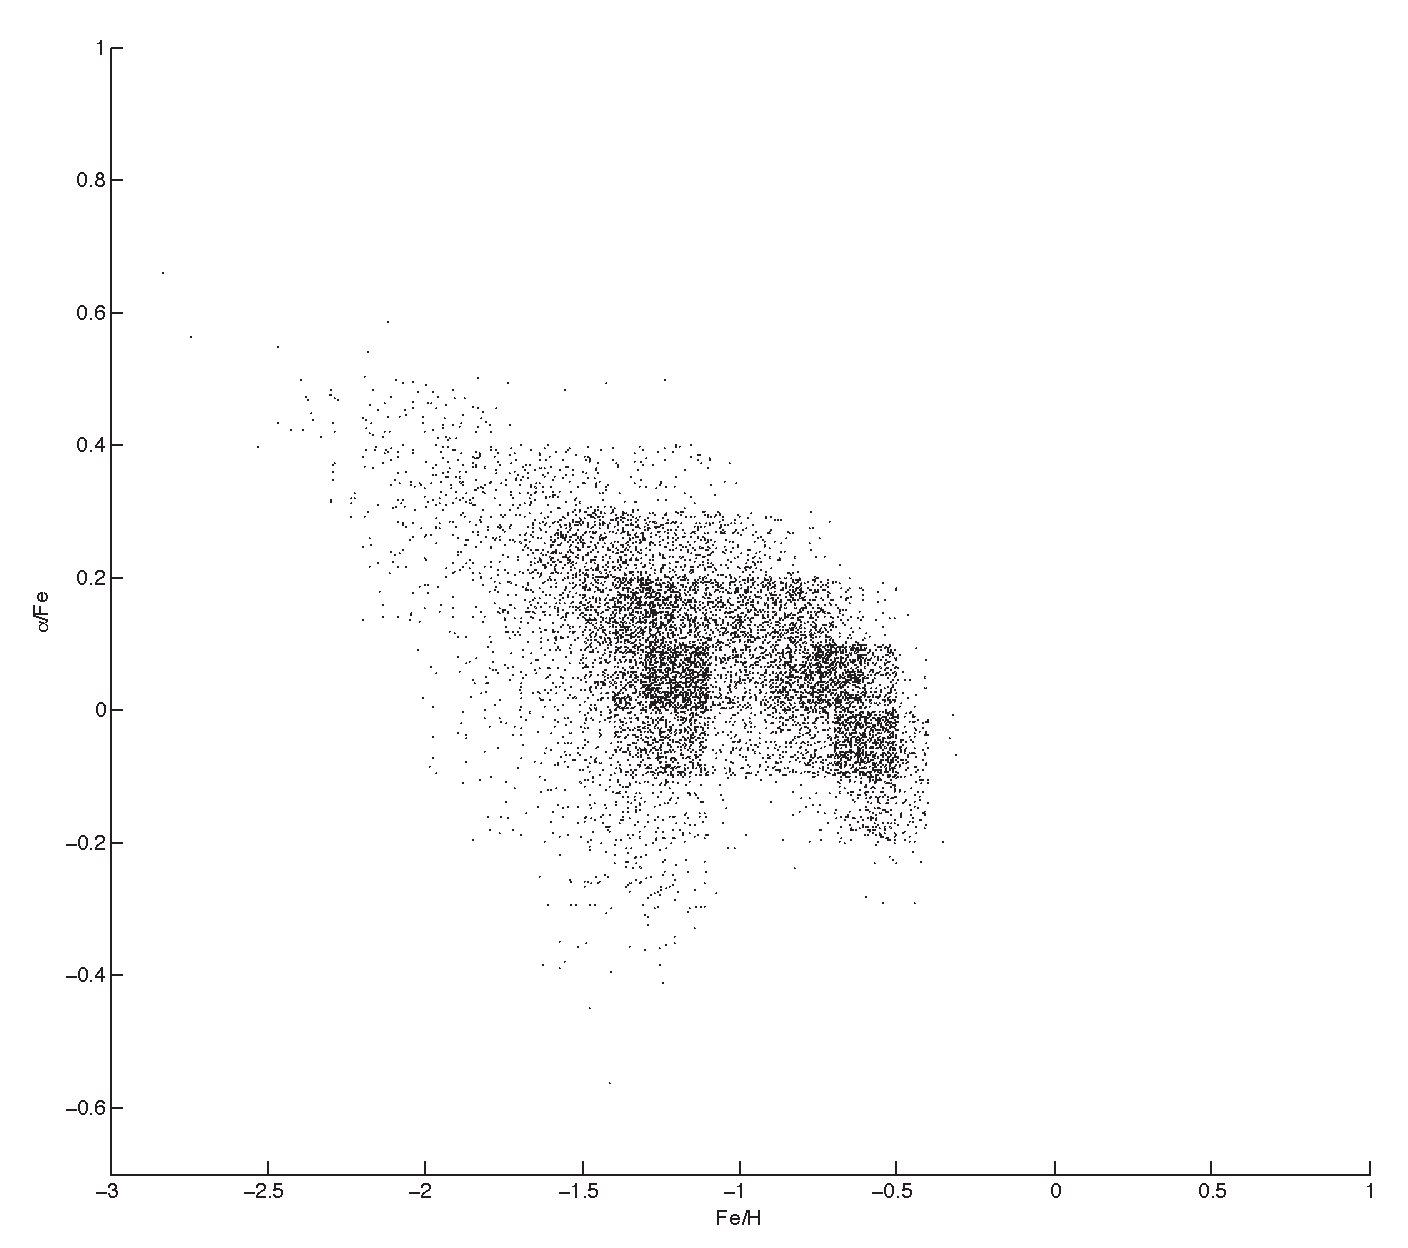
\includegraphics[width=0.4\textwidth]{boot_gen_data.pdf}
  \end{center}
  \caption{Generated parametrically}
\end{wrapfigure}

Given a $\vph$ from the EM algorithm, we can construct $B$ bootstrapped samples by plugging-in $\vph$ into our mixture model. Using uniform random numbers we first pick the $\pi_j$ from which to sample from, and then, from that $\pi_j$, we use another random number generator to pick a point on the CDF of the model data for the $\pi_j$. We then add noise so as to uniformly randomly distribute the pick over the grid specified in the model data.




\subsection{Non-Parametric data generation}
An alternate approach is to resample the given dataset directly, without relying on a mixture model. We sample, with replacement, $n$ data points from our original $n$ data points, where each data point is equally likely to be picked.





\subsection{Confidence intervals for $\vph$}

Given $B$ bootstrap estimates, $\vph^*_1,\ldots,\vph^*_B$, confidence intervals for each $\pi_j$ can be constructed based on $\hat{\pi}^*_j \xrightarrow{d} \hat{\pi}_j$. Instead we use a centered and scaled approach based on the central limit theorem:
\eqn{
	\sqrt{n}(\hat{\pi}_j - \pi_j) \xrightarrow{d} \script{N}(0,\sigma_j)
}

Thus the $1-\alpha$ confidence interval is bounded by $q_{\alpha/2}$ and $q_{1-\alpha/2}$ such that

\eqn{
	P\bl q_{\alpha/2} \leq \sqrt{n}(\hat{\pi}_j - \pi_j) \leq q_{1-\alpha/2} \br &= 1-\alpha	
}


and since

\eqn{
	\sqrt{n}(\hat{\pi}_j - \pi_j) \approx \sqrt{n}(\hat{\pi}^*_j - \hat{\pi}_j)
}

The $1-\alpha$ bootstrapped confidence interval is bounded by $q^*_{\alpha/2}$ and $q^*_{1-\alpha/2}$ such that

\eqn{
	P\bl q^*_{\alpha/2} \leq \sqrt{n}(\hat{\pi}^*_j - \hat{\pi}_j) \leq q^*_{1-\alpha/2} \br & \approx 1-\alpha	
}

Therefore confidence intervals can be computed as
\eqnl{sccib}{
	\hat{\pi}_j - \frac{q^*_{1-\alpha/2}}{\sqrt{n}} \leq \pi_j \leq \hat{\pi}_j - \frac{q^*_{\alpha/2}}{\sqrt{n}}
}

\subsection{Covariance, correlation, and standard deviation}
The covariance matrix of the bootstrap estimates can be approximated by the sample covariance:

\eqnl{scvmn}{
	\text{Covar}^*(\hat{\pi}_i,\hat{\pi}_j) = \frac{1}{B-1} \sum^B_{b=1} (\hat{\pi}_{bi}^*-\bar{\pi}_i)(\hat{\pi}_{bj}^*-\bar{\pi}_j)
}
where
\eqn{
	\bar{\pi}_i = \frac{1}{B}\sum_{b=1}^B \hat{\pi}^*_i
}


With a standard deviation of
\eqn{
	\hat{\sigma}^*_i &= | \text{Covar}^*(\hat{\pi}^*_i,\hat{\pi}^*_i)|	\\
}

the sample correlation matrix is given by
\eqnl{scmb}{
	\rho^*(\pi_i,\pi_j) &= \frac{\text{Covar}^*(\hat{\pi}_i,\hat{\pi}_j)}{\hat{\sigma}^*_i \hat{\sigma}^*_j}
}


\begin{figure}[h!]
  \centering
    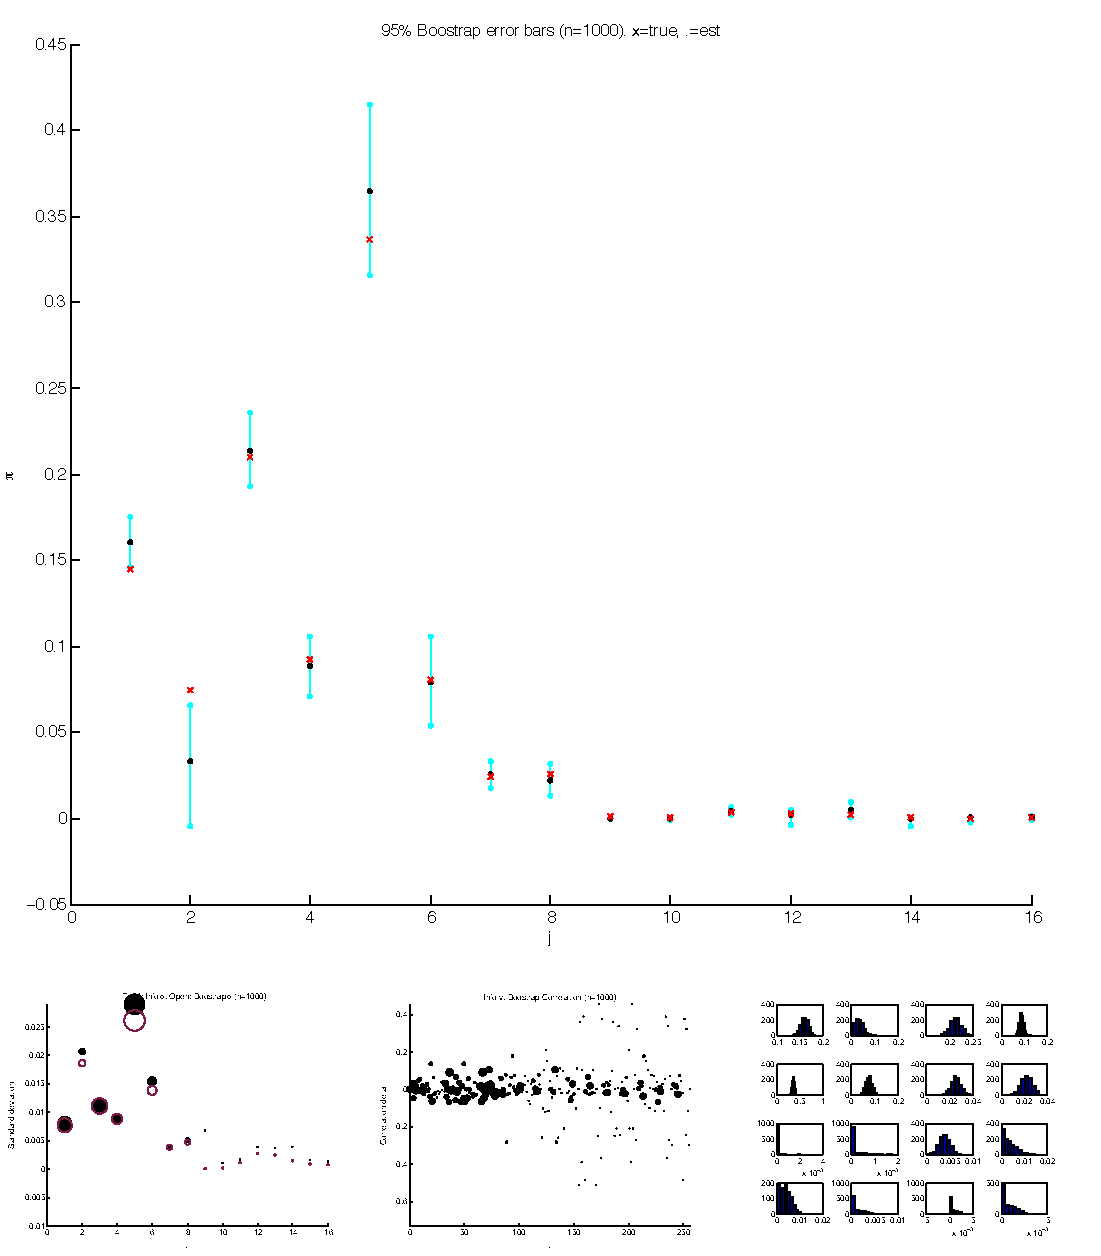
\includegraphics[width=1.1\textwidth]{mn_bootstrap.pdf}
    \caption{95\% bootstrapped confidence interval for n-out-of-n non-parametric resampling. Comparisons with information based confidence intervals below.}
\end{figure}


\begin{figure}[h!]
  \centering
    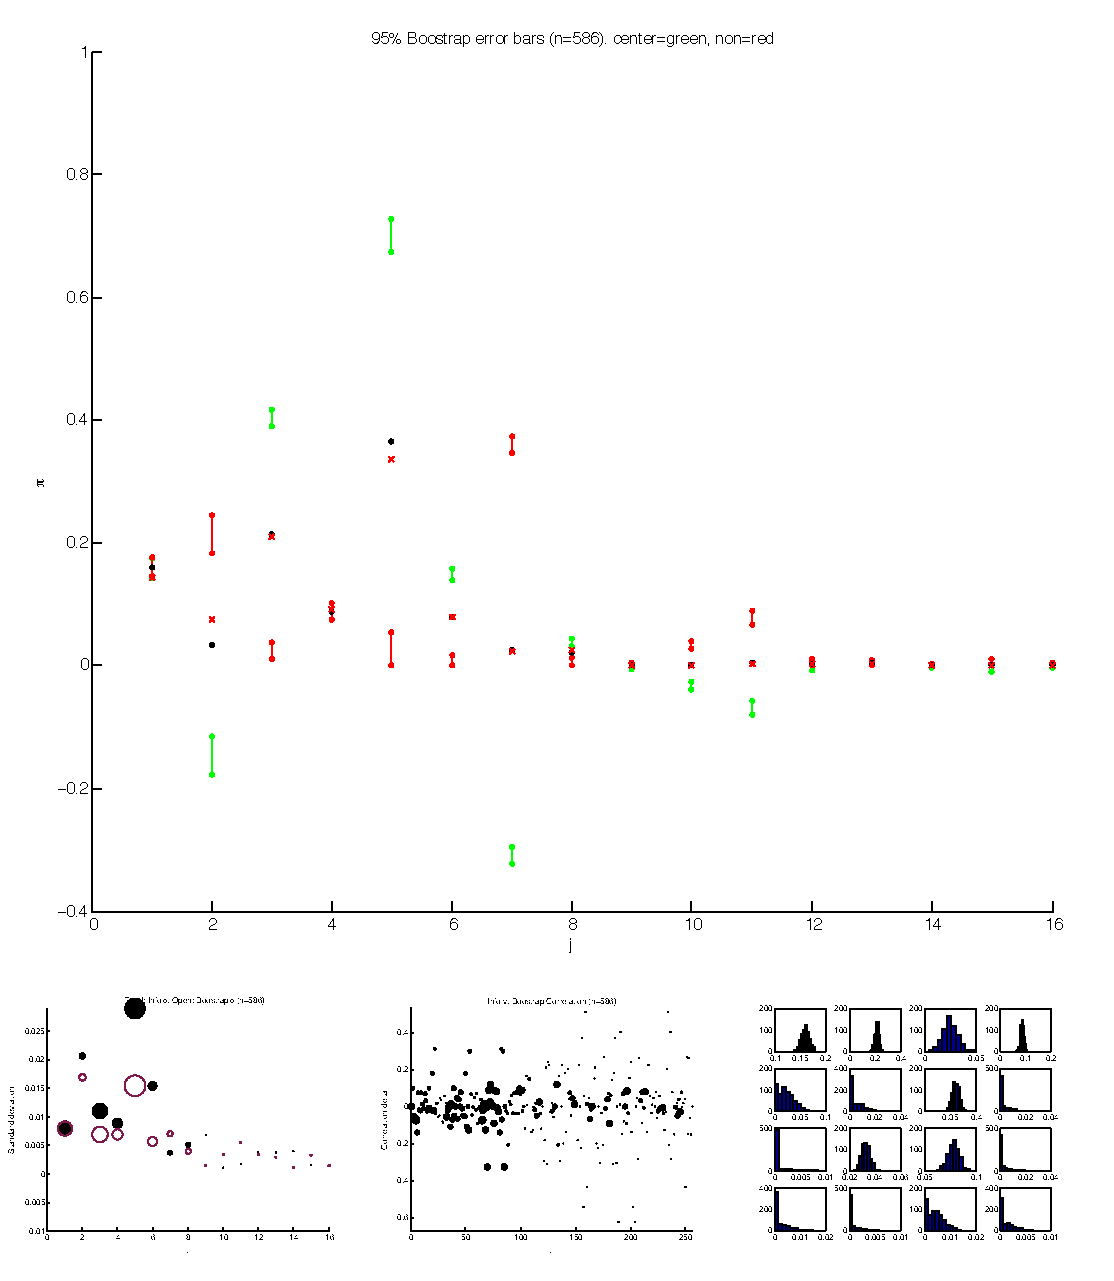
\includegraphics[width=1.1\textwidth]{g_bootstrap.pdf}
    \caption{95\% bootstrapped confidence interval for generated parametric resampling. Green bars are centered, red bars are non-centered. Comparisons with information based confidence intervals below.}
\end{figure}


\begin{figure}
	
	\begin{center}
		\includegraphics[scale=.75]{correlation_bmn_3.png}
	\end{center}
	\caption{Left: correlation where size of sphere represents correlation value, and opacity of sphere represents $\pi_q+\pi_p$. Orange bubbles represent negative correlation, and blue positive. Right: Same graph, but without transparency.}
\end{figure}


\begin{figure}
	
	\begin{center}
		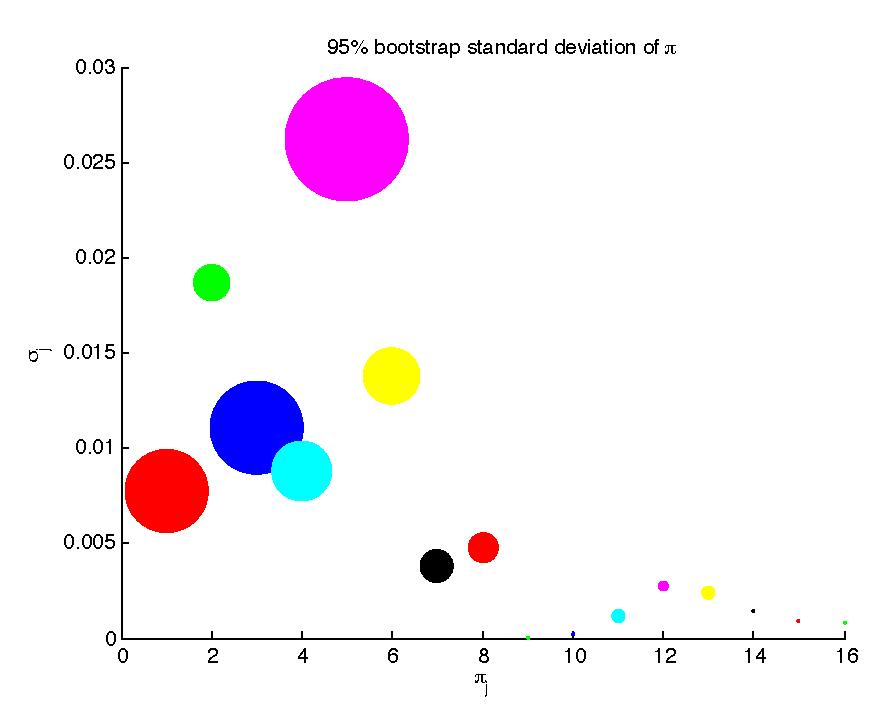
\includegraphics[scale=0.5]{boot_mn_stdev.pdf}
	\end{center}
	\caption{95\% n-out-of-n bootstrap standard deviation of each $\pi_j$.}
\end{figure}



\clearpage
\begin{table}[h]\tiny
\caption{95\% bootstrap correlation matrix}
	\begin{center}
		\noindent\makebox[\textwidth]{%
\begin{tabularx}{1.3\textwidth}{r| r r r r r r r r r r r r r r r r}
& 1 & 2 & 3 & 4 & 5 & 6 & 7 & 8 & 9 & 10 & 11 & 12 & 13 & 14 & 15 & 16	\\
\hline
   1   &         1   &    -0.582   &    -0.058   &    -0.174   &     0.258   &    -0.087    &     0.01    &   -0.054   &     0.005   &    -0.058   &     0.009   &    -0.027   &     0.027    &    0.003   &         0   &    -0.029      \\
   2   &    -0.582   &         1   &    -0.396   &     0.248   &     -0.62   &     0.314    &   -0.004    &    0.013   &     0.018   &     0.007   &     0.028   &     0.013   &    -0.036    &   -0.029   &    -0.043   &     0.017      \\
   3   &    -0.058   &    -0.396   &         1   &     0.142   &    -0.101   &    -0.129    &    -0.03    &    0.004   &     0.007   &     0.061   &    -0.075   &     0.023   &    -0.005    &    -0.01   &     0.071   &    -0.029      \\
   4   &    -0.174   &     0.248   &     0.142   &         1   &    -0.658   &      0.31    &   -0.159    &   -0.022   &    -0.022   &     0.054   &     0.015   &     0.014   &     0.008    &   -0.028   &    -0.013   &    -0.013      \\
   5   &     0.258   &     -0.62   &    -0.101   &    -0.658   &         1   &    -0.731    &    0.038    &    0.018   &    -0.023   &     -0.03   &    -0.021   &    -0.004   &     0.016    &    0.087   &     0.015   &     0.025      \\
   6   &    -0.087   &     0.314   &    -0.129   &      0.31   &    -0.731   &         1    &    0.001    &   -0.147   &     0.019   &     0.019   &     0.011   &     0.006   &    -0.045    &   -0.207   &     -0.02   &    -0.064      \\
   7   &      0.01   &    -0.004   &     -0.03   &    -0.159   &     0.038   &     0.001    &        1    &   -0.627   &     0.057   &    -0.036   &    -0.051   &     -0.07   &     0.084    &   -0.032   &    -0.007   &     0.029      \\
   8   &    -0.054   &     0.013   &     0.004   &    -0.022   &     0.018   &    -0.147    &   -0.627    &        1   &    -0.032   &    -0.024   &     0.125   &    -0.261   &    -0.037    &     0.08   &     0.035   &     0.005      \\
   9   &     0.005   &     0.018   &     0.007   &    -0.022   &    -0.023   &     0.019    &    0.057    &   -0.032   &         1   &    -0.001   &    -0.053   &     0.014   &    -0.001    &   -0.021   &     0.038   &     -0.03      \\
   10   &   -0.058   &     0.007   &     0.061   &     0.054   &     -0.03   &     0.019    &   -0.036    &   -0.024   &    -0.001   &         1   &    -0.156   &     0.125   &    -0.176    &    -0.01   &     0.051   &    -0.055      \\
   11   &    0.009   &     0.028   &    -0.075   &     0.015   &    -0.021   &     0.011    &   -0.051    &    0.125   &    -0.053   &    -0.156   &         1   &    -0.373   &     0.046    &    0.056   &    -0.173   &    -0.048      \\
   12   &   -0.027   &     0.013   &     0.023   &     0.014   &    -0.004   &     0.006    &    -0.07    &   -0.261   &     0.014   &     0.125   &    -0.373   &         1   &     -0.54    &   -0.013   &      0.04   &     0.089      \\
   13   &    0.027   &    -0.036   &    -0.005   &     0.008   &     0.016   &    -0.045    &    0.084    &   -0.037   &    -0.001   &    -0.176   &     0.046   &     -0.54   &         1    &   -0.064   &    -0.327   &    -0.107      \\
   14   &    0.003   &    -0.029   &     -0.01   &    -0.028   &     0.087   &    -0.207    &   -0.032    &     0.08   &    -0.021   &     -0.01   &     0.056   &    -0.013   &    -0.064    &        1   &    -0.063   &    -0.132      \\
   15   &        0   &    -0.043   &     0.071   &    -0.013   &     0.015   &     -0.02    &   -0.007    &    0.035   &     0.038   &     0.051   &    -0.173   &      0.04   &    -0.327    &   -0.063   &         1   &    -0.087      \\
   16   &   -0.029   &     0.017   &    -0.029   &    -0.013   &     0.025   &    -0.064    &    0.029    &    0.005   &     -0.03   &    -0.055   &    -0.048   &     0.089   &    -0.107    &   -0.132   &    -0.087   &         1      \\
\end{tabularx}}
	\end{center}
\end{table}



\end{document}

















